\documentclass{article}
\usepackage{ctex}
\usepackage{amsmath}
\usepackage{graphicx}
\usepackage{wrapfig}
\usepackage{caption}
\usepackage[top=0.8in, bottom=0.8in,left=0.8in, right=0.8in]{geometry}
\usepackage{float} 
\usepackage{subfigure}
\usepackage{subcaption}
\usepackage{bm}
\xeCJKsetup{CJKmath=true} 
\title{\textbf{第一届$\Sigma Pho$物理竞赛试题}}
\date{2023年11月}
\begin{document}
\maketitle
\begin{flushright}
    命题:胡锦浩,盛铖开、应佑、李骏亭\\
	审题,组题:胡锦浩
\end{flushright}
$$\textbf{考生必读}$$
\begin{itemize}
\item[1.]\textbf{考生考试前请务必阅读本须知。}
\item[2.]\textbf{本试题共 7 题,满分 320 分。}
\item[3.]\textbf{如遇到试题印刷不清楚的情况,请向监考老师提出。}
\item[4.]\textbf{需要阅卷老师评阅的内容一定要写在答题纸相应题号后面的空白处;阅卷老师只评阅答题纸上的内容,写在试题纸和草稿纸上的内容一律不被评阅。}
\end{itemize}

\section*{第一题、简单光学题(40分)}
\begin{itemize}
\item[(1)]一宽平行光束正入射到折射率为$n$的平凸透镜左侧平面,汇聚到平凸透镜主轴上的$F$点,已知$\overline{OF}=r_0$给出凸面型状,并给出其在直角坐标系下的标准方程,(需声明原点)。
\item[(2)]磁场透镜\par
一宽束质量,速度,电荷量分别为$m,v,q$入射到$x=0$平面。已知在第一、四象限存在大小为$B$,方向相反的磁场区域,出射后汇聚于$F(f,0)$处,给出磁场区域边界方程。
\item[(3)]电场透镜\par
一宽束质量,速度,电荷量分别为$m,v,q$入射到$x=0$平面。全空间中分布着如下电场
\[
\vec{E}=
\begin{cases}
-ky^{\alpha}\hat{y}(y>0)\\
ky^{\alpha}\hat{y}(y<0)
\end{cases}
\]
出射后汇聚于$F(f,0)$处,通过一些性质给出$\alpha$,并给出$k$的定量表达式。
\item[(4)]正经光学题\par
一束光平行于$x$轴方向入射,第一、四象限存在折射率只与$y$有关的介质,其边界是锯齿状的,使得光能垂直接着入射,出射后汇聚于$F(f,0)$处,在$(0,0)$处折射率为$n_0$,类比$(3)$给出折射率分布与边界方程.
\end{itemize}
\clearpage
\section*{第二题、悬链线(40分)}
\begin{wrapfigure}{r}{7cm}
	\vspace{-15pt}    % 对应高度1
	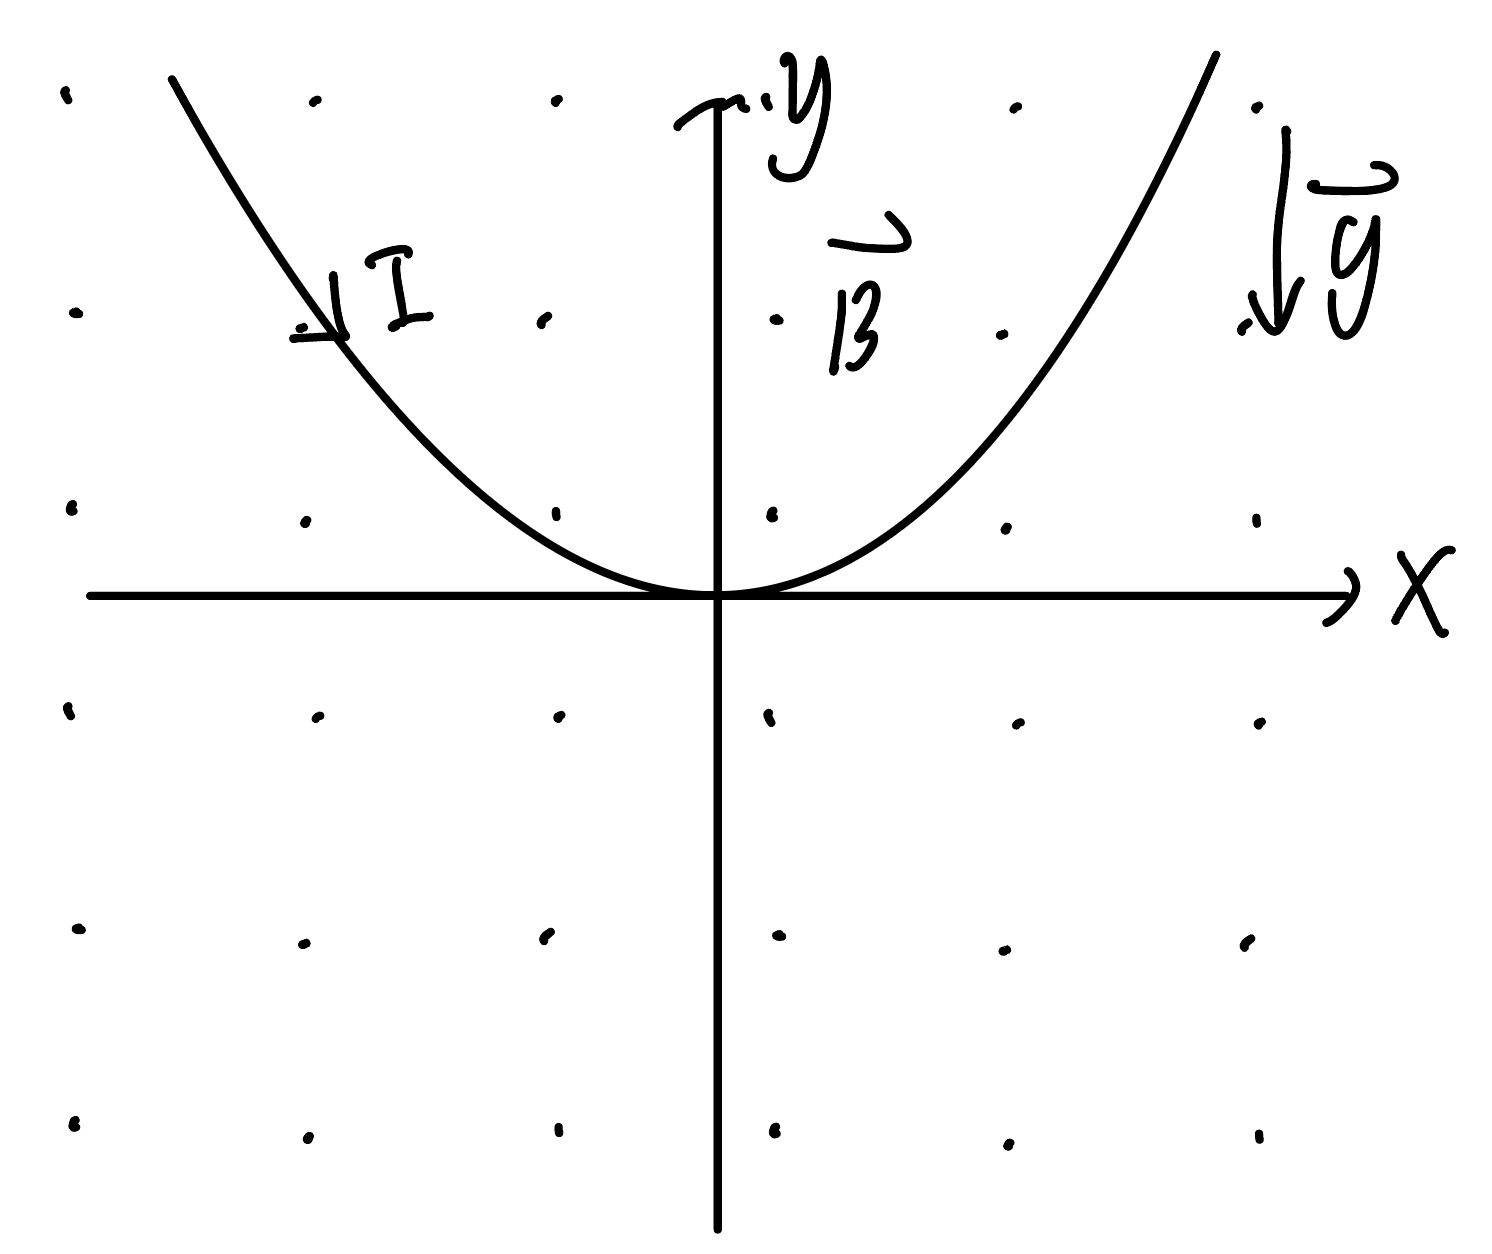
\includegraphics[width=7cm]{img/2.1.jpeg}\\
	\vspace{-15pt}    % 对应高度2
	\vspace{-15pt}    % 对应高度3
\end{wrapfigure}
竖直平面内挂有一根柔软的质量线密度为$\lambda$的均匀导线,其中通有电流$I$,存在如图所示的匀强磁场$B$,重力场$g$
已知底部$(x,y)=(0,0)$处张力为$T_0$。
试求其形状的微分方程,用$\mathrm{d}x,\mathrm{d}y$表示
\begin{itemize}
\item[(1)]取$B=0$,求其轨迹方程。\par
    注:双曲函数定义
    $$
    \cosh(x)=\dfrac{\mathrm{e}^{x}+\mathrm{e}^{-x}}{2},\sinh(\theta)=\dfrac{\mathrm{e}^{x}-\mathrm{e}^{-x}}{2}
    $$
\item[(2)]取$g=0$,求其轨迹方程。
\item[(3)]试求其形状的微分方程,用$\mathrm{d}x,\mathrm{d}y$表示.  
\end{itemize}

\section*{第三题、液体表面张力系数的确定(40分)}
众所周知液体有表面张力,但是往往表面张力系数是由实验测定的,下尝试通过理论方式建立。\par
\begin{itemize}
\item[(1)]已知热力学第一定律的微分形式是$\mathrm{d}U=Y\mathrm{d}y+T\mathrm{d}s$,其中$Y$是广义力,$y$是广义坐标,给出表面张力系统的热力学第一定律的微分形式。
\end{itemize}\par
液体内部的分子,其周围所受的力在平均后是各向同性的,但在液体表面,由于上面部分没有液体分子。用“作用力球”来说明,就是液体内部“作用力球”完整,而在表面“作用力球”少了一个球冠,从而导致了其受力并不为零,下给出定量分析的模型。\par
计液体内任意两个相邻的分子之间的相互作用能为$\varepsilon$,且液体内部一个分子与$n$个分子相邻,在表面与$\zeta n$个分子相邻.
\begin{itemize}
\item[(2)]给出内外分子势能的差值。
\item[(3)]设表面的粒子面密度为$\sigma_n$,求形成$\mathrm{d}A_S$面积的表面时做的功,并用$\sigma_n,\varepsilon,n,\zeta$表示表面张力系数$\sigma$。\par
\end{itemize}
\par
下确定$\varepsilon$.考虑液体汽化过程,给出摩尔汽化热$L_m$(认为是从内部分子汽化出去的).
\begin{itemize}
\item[(4)]给出$\varepsilon$,用$L_m,N_A,n$表示表面张力系数。
\item[(5)]认为一个分子占据半径为$d$的空间,给出液体分子的摩尔质量$\mu$和密度$\rho$,用$\zeta,L_m,N_A,\rho,\mu$表示表面张力系数$\sigma$ 
\end{itemize}
\par
现考虑混合液体的表面张力系数,设液体的两种组分为$\mu_1,\rho_1,d_1,n_1,\zeta_1,\sigma_{n_1}$和$\mu_2,\rho_2,d_2,n_2,\zeta_2,\sigma_{n_2}$,其中$n$数密度,液体内两种组分每个分子与均与$x_1,x_2$个分子相邻。两种组分之间的相互作用能为$\varepsilon_{11},\varepsilon_{22},\varepsilon_{12}$,并假设$|\varepsilon_{12}|=\sqrt{|\varepsilon_{11}||\varepsilon_{22}|}$
\begin{itemize}
\item[(6)]给出混合液体的表面张力系数$\sigma_{12}$,用$\mu_1,\rho_1,d_1,n_1,\zeta_1,\sigma_{n_1},x_1,\mu_2,\rho_2,d_2,n_2,\zeta_2,\sigma_{n_2},x_2$
\end{itemize}

\section*{第四题、受限三体问题与拉格朗日点(60分)}
	对于任意给定的$m_1,m_2,m_3$,仅在万有引力的作用下运动,在任意给定初值的条件下求解$m_1,m_2,m_3$的运动的问题称作三体问题,时至今日依旧没有解析解,但对于$m_1,m_2\gg m$的情况下,且完全忽略$m$对$m_1,m_2$运动的影响,称为受限三体问题。\par
	在这类问题中,有一些点满足在$m_1,m_2$公转系中静止的条件,这些点称为拉格朗日点。\par
	下认为$m_1,m_2$均作圆周运动,以质心为原点,$(r_1,0)$表示$m_1$的位置,$(-r_2,0)$表示$m_2$的位置,且$r=r_1+r_2$。\par
\begin{itemize}
\item[(1)]	给出任意$(x,y)$处的有效势.(单位质量势能,$m_1,m_2$除外)
\item[(2)]	给出拉格朗日点满足的方程(无需求解)给出$y=0$拉格朗日点的个数,并定性描述其位置.\par
在一定近似下,我们可以求解,如令
$$\varepsilon=\dfrac{m_1}{m_2}\to 0.$$
\item[(3)]	给出$y=0$时的零阶解,并进一步描述位置.
\item[(4)]	给出$y=0$时的一阶解,并给出坐标.
\item[(5)]	求出剩下的点,并指出其特殊几何关系.
\end{itemize}

\section*{第五题、匀强磁场中带电小球在圆盘上的运动(50分)}
\begin{wrapfigure}{r}{7cm}
	\vspace{-15pt}    % 对应高度1
	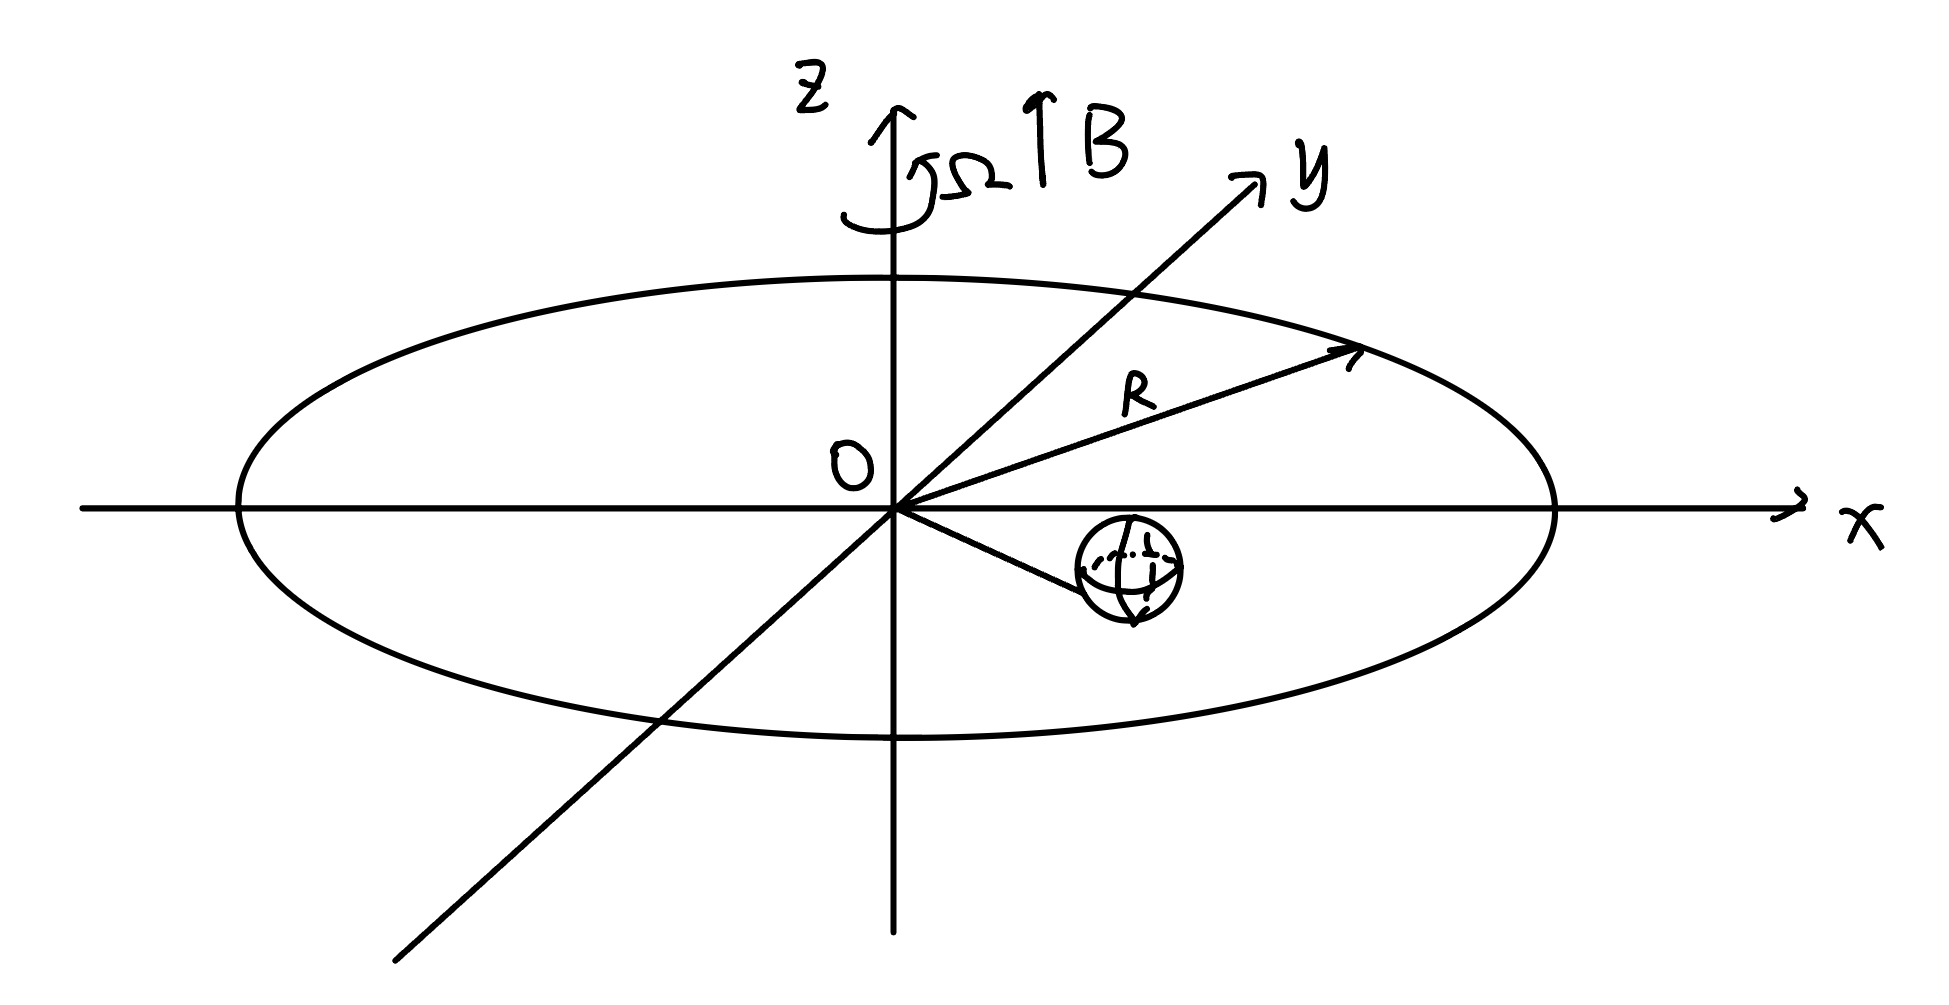
\includegraphics[width=7cm]{img/5.1.jpeg}\\
	\vspace{-15pt}    % 对应高度2
	\vspace{-15pt}    % 对应高度3
\end{wrapfigure}
考虑一个沿$z$轴以匀角速度$\Omega$转动的薄圆盘半径为$R$,质量为$M$。有一半径为$r$,均匀带电量为$Q$,质量为$m$的小球,小球与圆盘间无滑动。全空间存在竖直向上的匀强磁场,大小为$B$.\par
初始将小球静止放在$(r_0,0,0)$处,考虑其运动。\par
\begin{itemize}
\item[(1)]当带电小球以$\vec{\omega}$转动时,求带电小球的总磁矩$\vec{\mu}$。\par
注:磁矩定义$\vec{\mu}=I\vec{S}$\par
\item[(2)]初始$t=0$,求解之后的运动。
\end{itemize}

\section*{第六题、Arago圆盘(40分)}
\begin{wrapfigure}{r}{7cm}
	\vspace{-15pt}    % 对应高度1
	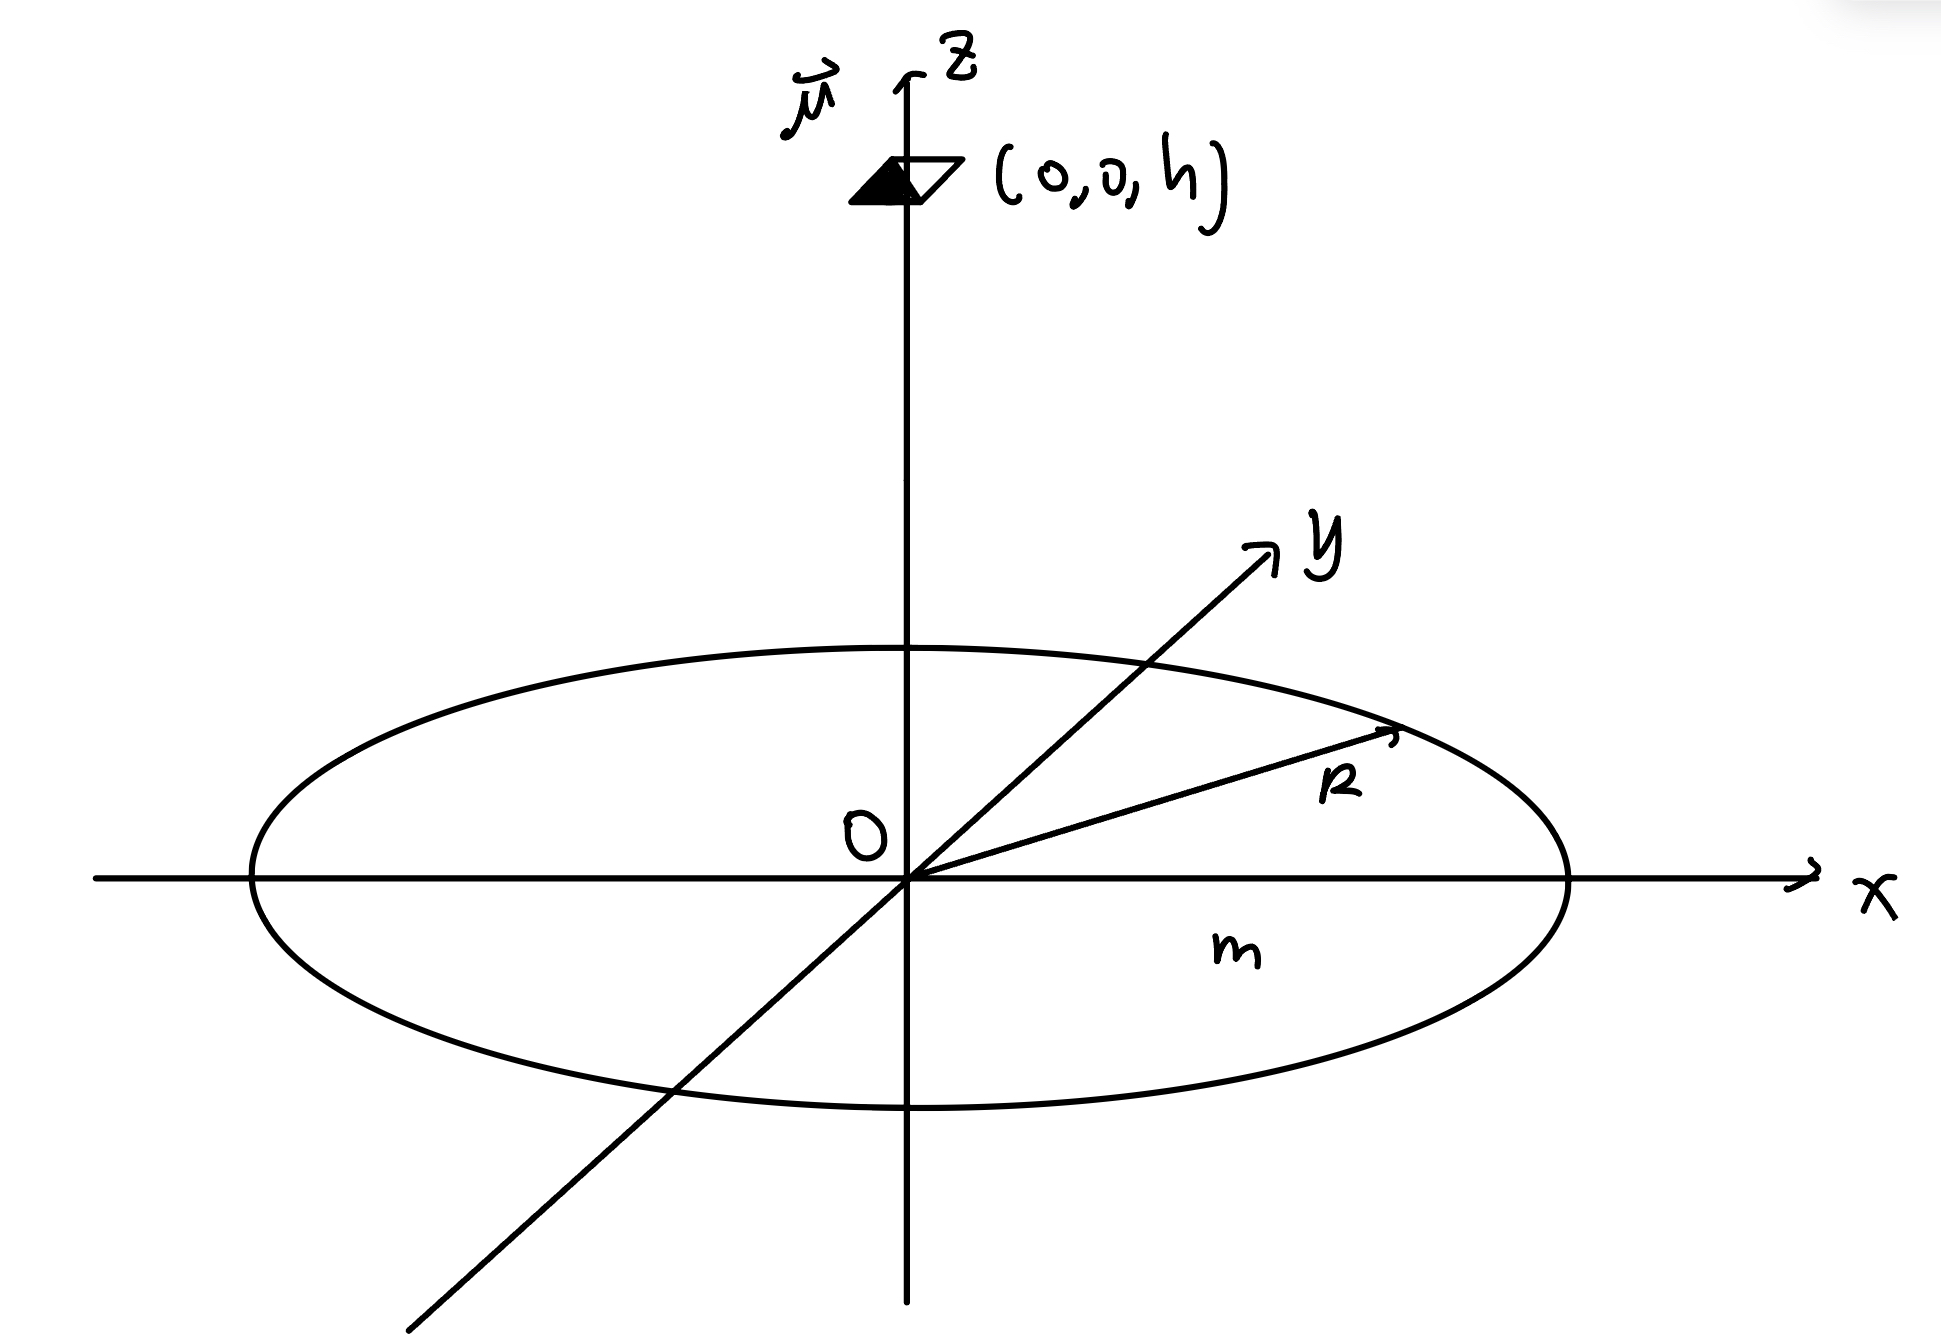
\includegraphics[width=7cm]{img/6.1.jpeg}\\
	\vspace{-15pt}    % 对应高度2
	\vspace{-15pt}    % 对应高度3
\end{wrapfigure}
高二这次期中考考了一个有关于Arago圆盘的选择题,小H同学对J老师的解释不是很满意,于是他尝试自己着手计算一下。\par
将小磁针认为是一个磁偶极子,大小为$\mu$。下方$h$处有一个带电薄圆盘质量为$m$,半径为$R$,以$\omega$转动。
\begin{itemize}
    \item[(1)]现固定小磁针,将下方带电薄圆盘以$\Omega$恒定速度转动,求小磁针受到的力矩。
    \item[(2)]现释放小磁针,并解除下方维持带电薄圆盘匀速转动的力矩,求两者共速后的共同角速度$\Omega$.
\end{itemize}
补充:磁偶极子的场
\[
\vec{B}=\dfrac{\mu}{4\pi}\dfrac{(3(\vec{\mu}\cdot\hat{r})\hat{r}-\vec{\mu})}{|\vec{r}|^3}
\]
\section*{第七题、“简单力学题”(50分)}
\begin{wrapfigure}{r}{4cm}
	\vspace{-15pt}    % 对应高度1
	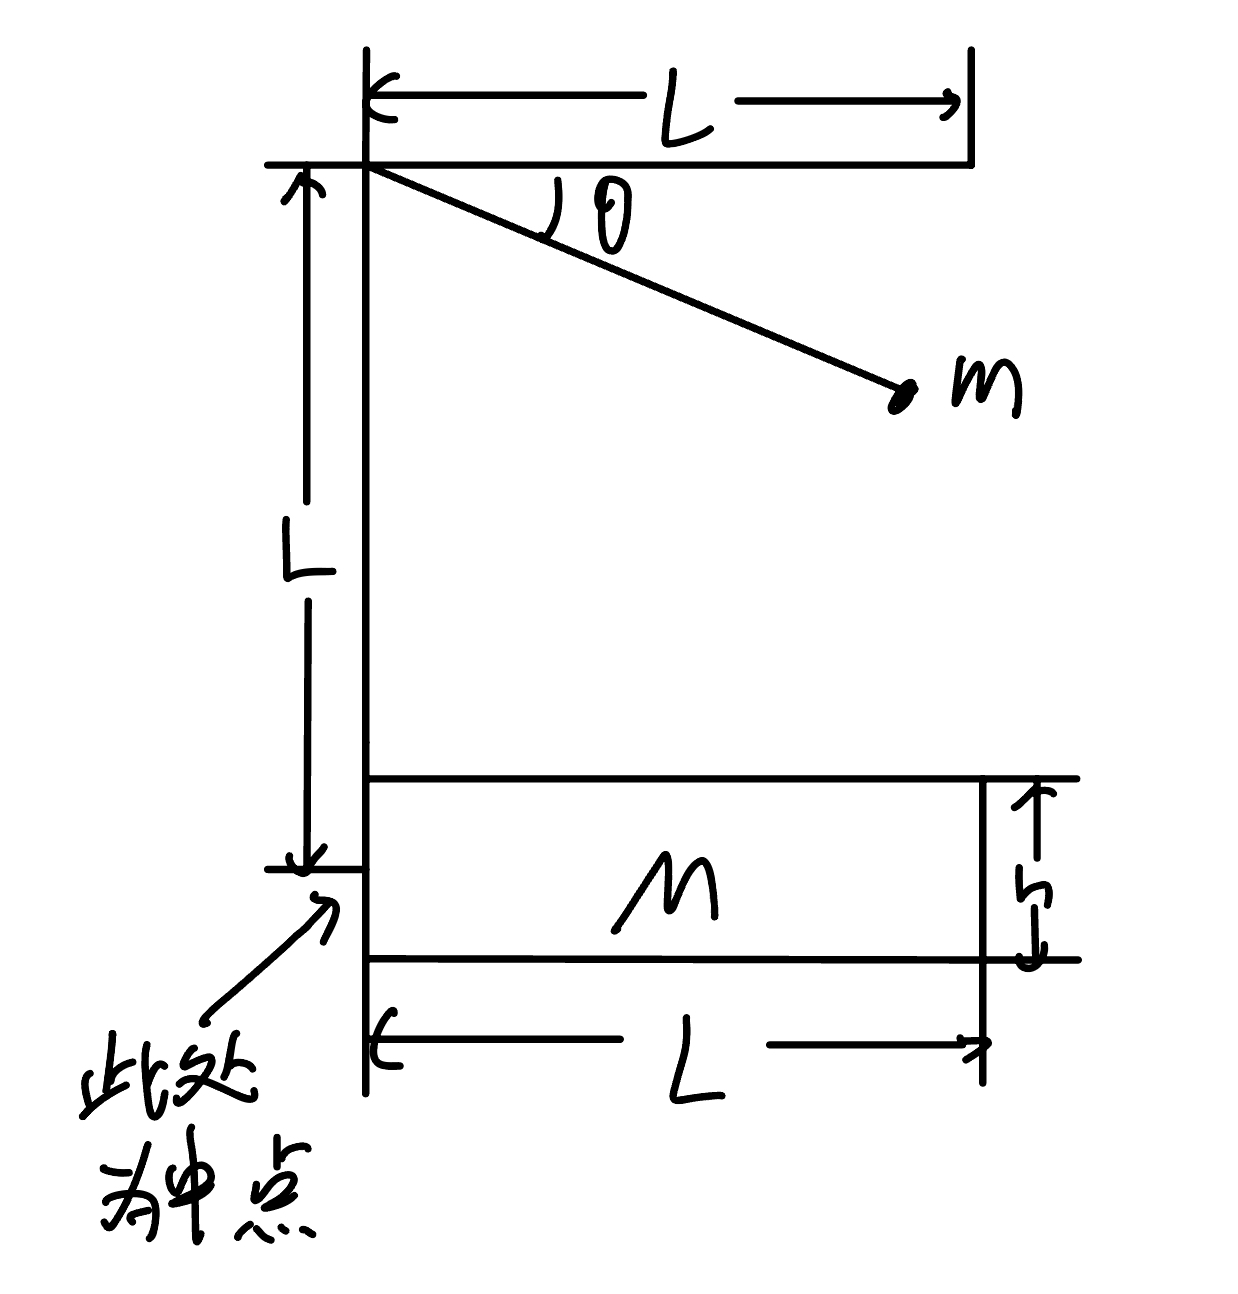
\includegraphics[width=4cm]{img/7.1.jpeg}\\
	\vspace{-15pt}    % 对应高度2
	\vspace{-15pt}    % 对应高度3
\end{wrapfigure}
光滑水平面上有一木块,匀质质量为$M$,在左端中间固定有一档板,其上有一绳,一侧系有一质量为$m$得质点。其中各参数如图所示,初态均静止,细绳水平释放质点。
试就$\frac{M}{m}=1,\frac{1}{2}$时,求木块右侧是否会离开地面。若会,其第一次离开时的$\theta$ .

\end{document}